\documentclass[11pt]{amsart}

% Standard letter size paper with 1inch margins
\usepackage[letterpaper, margin=1in]{geometry}

% Useful packages 
\usepackage{amsmath, amssymb, amsthm, amsaddr}
\usepackage{enumerate, subcaption, graphicx, hyperref}
\usepackage{algorithm}
\usepackage{algpseudocode}
\usepackage{cite}
\usepackage{titling}

% Custom math commands
\newcommand{\I}{\mathrm{i}}
\DeclareMathOperator{\E}{e}

% Title block
\title{HMS 581 Final Project}
\newcommand{\subtitle}{\large Modeling Measles in New York \& Vermont}
\author{Hunter Lybbert}
\address{Applied Mathematics Department, University of Washington, Seattle, WA 
\\ \texttt{hlybbert@uw.edu}}
\date{\today}

% Add subtitle formatting
\pretitle{\begin{center}\LARGE}
\posttitle{\par\medskip\subtitle\end{center}}
\preauthor{\begin{center}
\normalsize \lineskip 0.5em%
\begin{tabular}[t]{c}}
\postauthor{\end{tabular}\end{center}}
\predate{\begin{center}\small}
\postdate{\end{center}}

\begin{document}

\begin{center}
    {\LARGE \textbf{HMS 581 Final Project}}\\[1ex]
    {\large Modeling Measles in New York \& Vermont}\\[4ex]
    {\Large Hunter Lybbert}\\[2ex]
    \textit{Applied Mathematics Department, University of Washington, Seattle, WA}\\[1ex]
    \texttt{hlybbert@uw.edu}\\[1ex]
    \today
\end{center}

\vspace{2ex}
\begin{quote}
A\textsc{bstract.}
\small We model the spread of the measles pathogen in New York and Vermont from \textbf{START\_DATE} to \textbf{END\_DATE} using an SIR model.
Our model has been augmented from a basic SIR model to incorporate annual seasonality, births and deaths, and a multi-year seasonality term for the strength of the strain of the pathogen.
To optimize and fit our model, we adapted to python, the R implementation of particle MCMC provided to us.
\end{quote}

\section{Introduction and Model Augmentations}\label{sec:augmentations}
The standard SIR model tracks the portion of or total number of people from the population which are 
\subsection{Seasonality}
\subsection{Birth Deaths}
\subsection{Pathogen Strength (Multi-year oscilations)}

\section{Model Fitting and Results}\label{sec:results}
\textbf{TODO:} Sumarize pMCMC and present plots

%\begin{figure}[h]
%	\centering
%	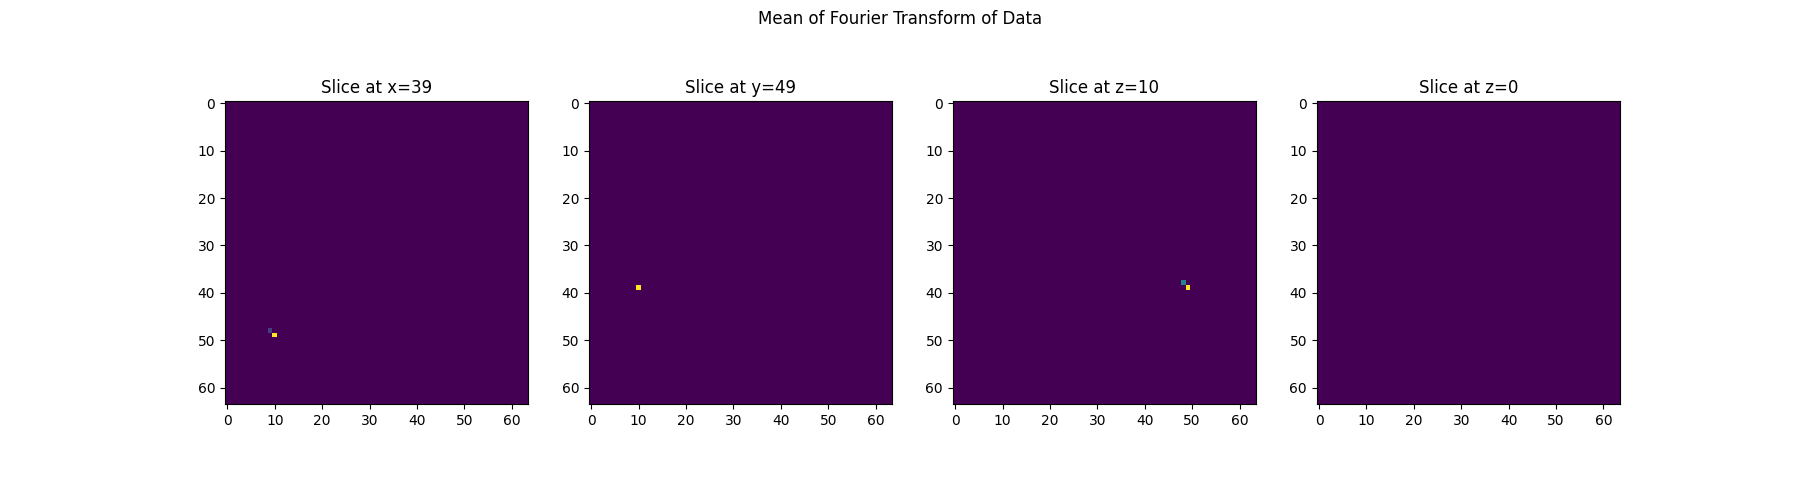
\includegraphics[width=1\textwidth]{../visualizations/visualizing_dominant_frequency.png}
% 	\caption{Visualizing each of the 3 slices including the location in our 3 dimensional average frequency object.}\label{fig:f1_0}
%\end{figure}
%
%\begin{figure}[h]
%	\centering
%	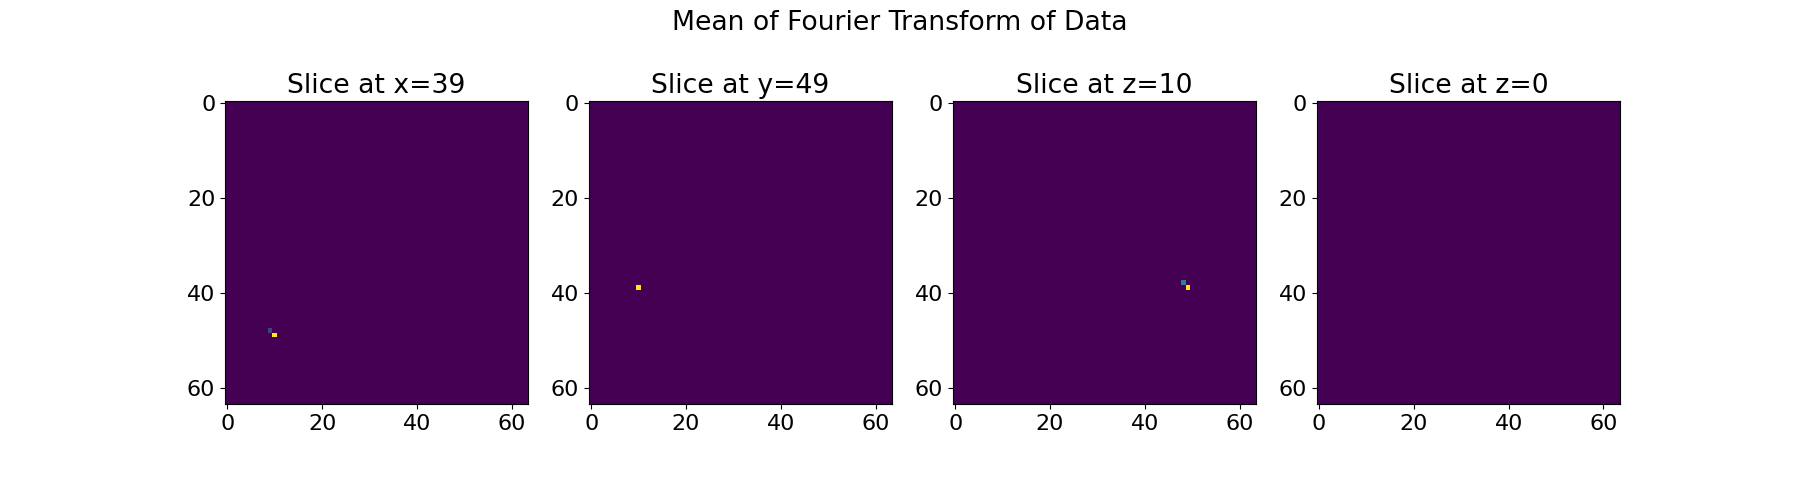
\includegraphics[width=1\textwidth]{../visualizations/visualizing_dominant_frequency_plus.png}
% 	\caption{Visualizing each of the 3 slices including the location in our 3 dimensional average frequency object. We also visualize a slice which does not intersect the max frequency in order to convey how drastic the location of the max frequency is. In order to show this comparison things have been rescaled here.}\label{fig:f1}
%\end{figure}

%\begin{figure}[h]
%	\centering
%	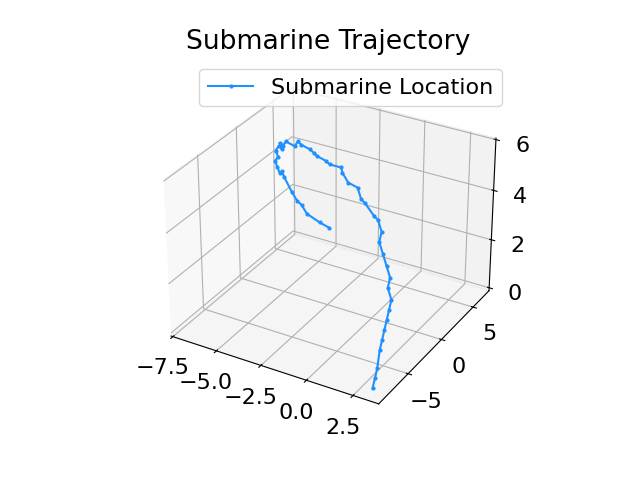
\includegraphics[height=2in]{../visualizations/submarine_static_3d.png}
% 	\caption{The resulting path in 3 dimensions that we determined after applying Algorithms \ref{alg:dom_freq} and \ref{alg:filter}. In this iteration of the filter we used $\sigma=1.3$.}\label{fig:f2}
%\end{figure}
%
%\begin{figure}[h]
%	\centering
%	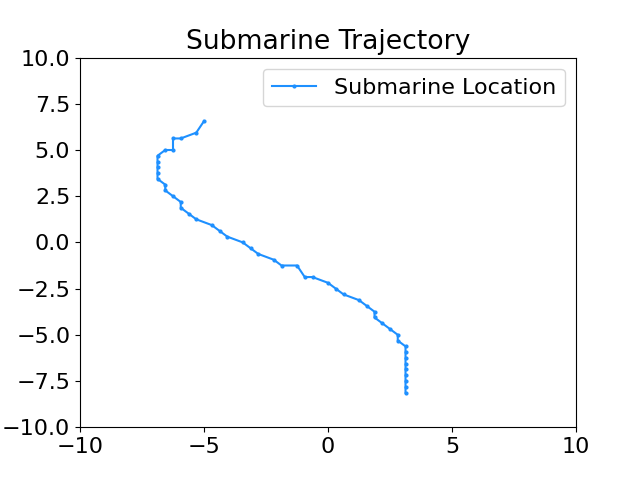
\includegraphics[height=2in]{../visualizations/submarine_static_2d.png}
% 	\caption{This is just the 2 dimensional projection of the path given in the above 3d plot. The same value of $\sigma$ was used in the filter.}\label{fig:f3}
%\end{figure}

\section{Conclusion}\label{sec:conclustion}
\textbf{TODO:} summarize, discuss possible future work

\section*{Acknowledgements} 
We would like to thank Bobby Reiner for a very instructive course and giving us ample opportunities to apply the material we learned in the classroom.
We would like to acknowledge the assistants from Nate Ward, Jaxon Tuggle, and Hailey Sparks who were instrumental in brainstorming ideas, debugging code, and analyzing results together.

\newpage
\appendix

\section{Best Fit Statistics}
\textbf{TODO:} make a table of best fit parameters

\section{Code}
\textbf{TODO:} Link to the github page with the code


\bibliographystyle{abbrv}
\bibliography{references_hw1} % make sure this matches the .bib file for your corresponding document. You also have to maintain your references in the .bib file 

\end{document}
